
\subsubsection{08.11.14}

\begin{enumerate}
	\item Время начала и окончания собрания:
	16:00 - 20:00
	\item Цели собрания:
	\begin{enumerate}
		\item Необходимо разработать новые идеи создания МЗК, поскольку предыдущие варианты его реализации не были удачными.
		
		\item Начать создание механизма захвата подвихных корзин.
		
	\end{enumerate}
	
	\item Проделанная работа:
	\begin{enumerate}
		\item Были предложены следующие идеи конструкции МЗК:
		\begin{enumerate}
			\item Механизм, состоящий из двух вертикальных реек, способных опускаться на горизонтальную часть основания подвижной корзины, а затем раздвигаться в стороны, упираясь в бортики основания и надежно фиксируя корзину. Плюсы: компактность, простота конструкции. Минусом конструкции является то, что с ее помощью нельзя захватить больше одной корзины зараз (захватывать сразу несколько корзин выгодно в автономном периоде и в финале). Кроме того, для захвата корзины данным приспособлением необходимо точно прицеливаться, что усложняет его использование.
			
			\item Механизм, состоящий из двух балок, способных опускаться с двух сторон от подвижной корзины, а потом, поворачиваясь вокруг вертикальной оси, сдавливать основание корзины с двух сторон. Плюсы: балки возможно дополнительно удлиннить для того, чтобы можно было захватить две корзины одновременно, захват подвижной корзины данным механизмом осуществлять проще, поскольку к ней не нужно тщательно прицеливаться. Минусы конструкции: некомпактность, сложность (возможно, придется использовать несколько сервоприводов для опускания балок).
			
			\item Механизм, состоящий из двух балок, способных опускаться с двух сторон от подвижной корзины, а потом, поворачиваясь вокруг горизонтальной оси, параллельной центральной оси робота, сдавливать основание корзины с двух сторон. Этот вариант очень похож на предыдущий и имеет те же плюсы и минусы.
			
			\begin{figure}[H]
				\begin{minipage}[h]{0.2\linewidth}
					\center  
				\end{minipage}
				\begin{minipage}[h]{0.6\linewidth}
					\center{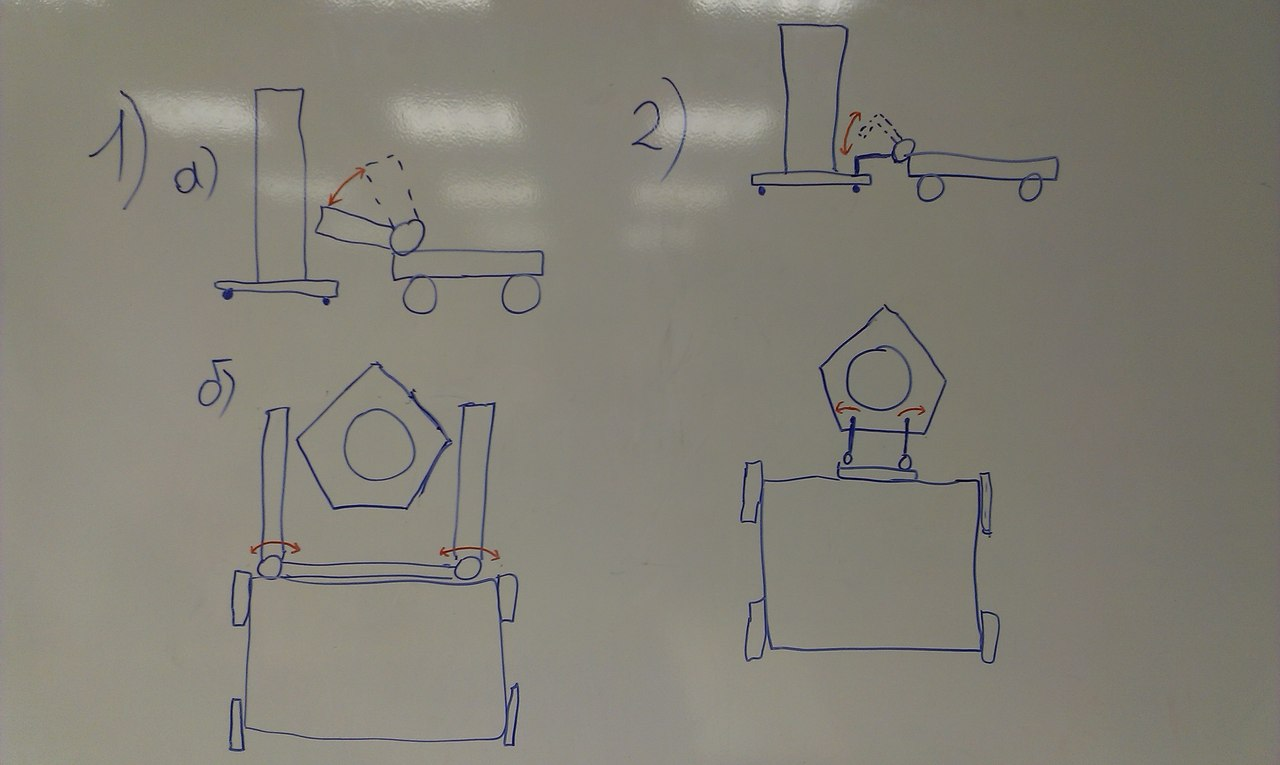
\includegraphics[scale=0.2]{days/08.11.14/images/01}}
					\caption{Идеи фиксирования подвижной корзины: 1)Клешни 2)Вертикальные рейки %-1 3)Клешни-2
						}
				\end{minipage}
			\end{figure}
			
		\end{enumerate}
		
		\item Поскольку механизм прицепа пока не был выбран, его сборка начата не была.
		
		\item Поскольку после того, как было решено отказаться от идеи МЗК с использованием сервопривода, поворачивающего балку, в задней детали робота осталось неиспользуемое отверстие, было решено приспособить его под гнездо для кнопки питания.
		
		\begin{figure}[H]
			\begin{minipage}[h]{0.2\linewidth}
				\center  
			\end{minipage}
			\begin{minipage}[h]{0.6\linewidth}
				\center{
\includegraphics[scale=0.2]{days/08.11.14/images/02}}
				\caption{Кнопка питания}
			\end{minipage}
		\end{figure}
		
	\end{enumerate}
	
	\item Итоги собрания: 
	\begin{enumerate}
		\item Предложено 3 идеи конструкции МЗК.
		
		\item Механизм захвата корзин не реализован.
		
	\end{enumerate}
	
	\item Задачи для последующих собраний:
	\begin{enumerate}
		\item Выбрать оптимальный вариант конструкции МЗК.
		
		\item Собрать МЗК.
		
	\end{enumerate}     
\end{enumerate}
\fillpage

